\documentclass[tikz,border=6pt]{standalone}
\usepackage[T1]{fontenc}
\usepackage{lmodern}
\usepackage{xcolor}

\definecolor{unmitigated}{HTML}{4C78A8}
\definecolor{mitigated}{HTML}{F58518}
\definecolor{reference}{HTML}{54A24B}
\definecolor{gridgray}{HTML}{D7DCE2}
\definecolor{textdark}{HTML}{20242A}

\begin{document}
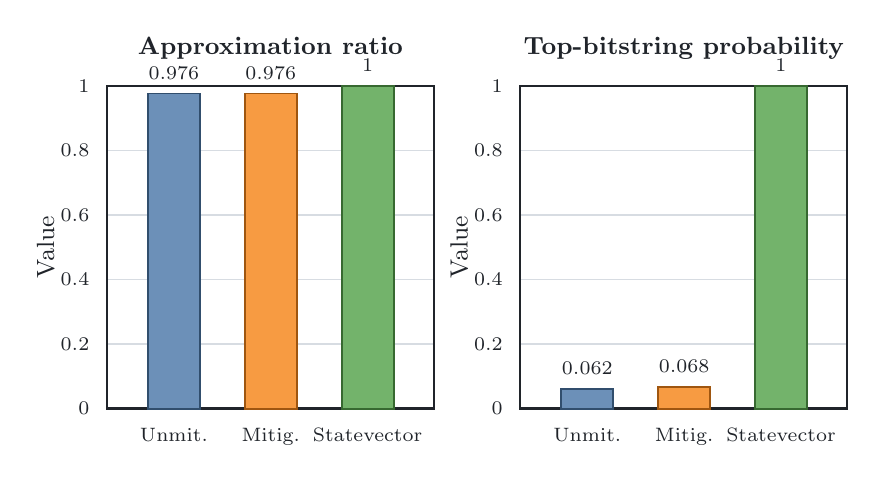
\begin{tikzpicture}[x=1cm,y=1cm,font=\sffamily,text=textdark]
  \def\panelwidth{4.15}
  \def\panelheight{4.1}
  \def\barwidth{0.66}

  \foreach \xshift/\title in {0/Approximation ratio,5.25/Top-bitstring probability} {
    \begin{scope}[xshift=\xshift cm]
      \foreach \v in {0,0.2,...,1.0} {
        \pgfmathsetmacro{\yy}{\v*\panelheight}
        \draw[gridgray,line width=0.45pt] (0,\yy) -- (\panelwidth,\yy);
        \node[anchor=east,font=\scriptsize] at (-0.10,\yy) {\pgfmathprintnumber[fixed,precision=1]{\v}};
      }
      \draw[textdark,line width=0.8pt] (0,0) rectangle (\panelwidth,\panelheight);
      \node[font=\small\bfseries] at (2.075,4.58) {\title};
      \node[rotate=90,font=\small] at (-0.78,2.05) {Value};
    \end{scope}
  }

  \foreach \x/\barvalue/\barcolor/\barlabel in {
    0.85/0.976/unmitigated/Unmit.,
    2.08/0.976/mitigated/Mitig.,
    3.31/1.000/reference/Statevector} {
    \pgfmathsetmacro{\height}{\barvalue*\panelheight}
    \filldraw[fill=\barcolor!82,draw=\barcolor!65!black,line width=0.7pt]
      (\x-0.33,0) rectangle (\x+0.33,\height);
    \node[anchor=south,font=\scriptsize\bfseries] at (\x,\height+0.06) {\pgfmathprintnumber[fixed,precision=3]{\barvalue}};
    \node[anchor=north,font=\scriptsize] at (\x,-0.12) {\barlabel};
  }

  \foreach \x/\barvalue/\barcolor/\barlabel in {
    6.10/0.062/unmitigated/Unmit.,
    7.33/0.068/mitigated/Mitig.,
    8.56/1.000/reference/Statevector} {
    \pgfmathsetmacro{\height}{\barvalue*\panelheight}
    \filldraw[fill=\barcolor!82,draw=\barcolor!65!black,line width=0.7pt]
      (\x-0.33,0) rectangle (\x+0.33,\height);
    \node[anchor=south,font=\scriptsize\bfseries] at (\x,\height+0.06) {\pgfmathprintnumber[fixed,precision=3]{\barvalue}};
    \node[anchor=north,font=\scriptsize] at (\x,-0.12) {\barlabel};
  }
\end{tikzpicture}
\end{document}